\section{From a regular expression to a finite state automaton}

There are a few algorithms to transform a regular expression into an automaton, which differ as for automaton characteristic. 

\subsection*{Thompson structural method}
Wit the Thompson structural method, given a regular expression, we analyze it into simple parts, we produce corresponding component automata, and we interconnect them 
to obtain the complete recognizer. In  this  construction each  component machine is  assumed to  have  exactly one initial state without incoming arcs and one final 
state without outgoing arcs. 
\begin{figure}[H]
    \centering
    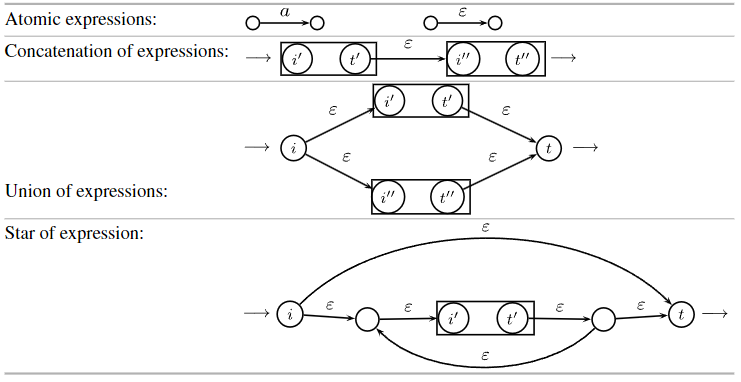
\includegraphics[width=1\linewidth]{images/thompson.png}
    \caption{Sub-expression to automaton}
\end{figure}
The validity of Thompson's method comes from it being an operational reformulation of the closure properties of regular languages under concatenation, union, and star.
In general the outcome of the Thompson method is a non-deterministic automaton with spontaneous moves. There are various optimizations of the Thompson method that avoid 
creating redundant states. 

\subsection*{Glushkov-McNaughton-Yamada algorithm}
The GMY algorithm constructs the automaton equivalent to a given regular expression, with states that are in a one-to-one correspondence with the generators that occur
in the regular expression. 

\begin{definition}
    Given a language $L$ over the alphabet $\Sigma$ we can define: 
    \begin{itemize}
        \item The set of initials: $Ini(L)=\{a \in \Sigma | a\Sigma^{*}\cap L \neq \varnothing\}$. 
        \item The set of finals: $Fin(L)=\{a \in \Sigma | \Sigma^{*}a\cap L \neq \varnothing\}$.
        \item The set of digrams: $Dig(L)=\{x \in \Sigma^{2} | \Sigma^{*}x\Sigma^{*} \cap L \neq \varnothing\}$.
        \item The set of forbidden digrams: $\overline{Dig(L)}=\Sigma^{2}-Dig(L)$
    \end{itemize}
    The language $L$ is called \emph{local} or \emph{locally testable}, if and only if it satisfies the following identity: 
    \[L-\{\varepsilon\}=\{x|Ini(x)\in Ini(L) \land Fin(x)\in Fin(L)\land Dig(x)\subseteq Dig(L)\}\]
\end{definition}
To design the recognizer of a local language we scan the input string from left to right and check whether: the initial character belongs to the set $Ini$, every 
digram belongs to the set $Dig$, and the final character belongs to the set $Fin$. The string is accepted if, and only if, all the above checks succeed. 

We can implement the above recognizer by resorting to a sliding window with a width of two characters, which is shifted over the input string from left to right.
At each shift step the window contents are checked, and if the window reaches the end of the string and all the checks succeed, then the string is accepted, otherwise
it is rejected. This sliding window algorithm is simple to implement by means of a non-deterministic automaton. 
\begin{definition}
    A regular expression is said to be \emph{linear} if there is not any repeated generator. 
\end{definition}
The idea of the GMY algorithm, based on the linear regular expressions is the following: 
\begin{enumerate}
    \item Denumerate the regular expression e and obtain the linear regular expression $e_{\#}$. 
    \item Compute the three characteristic local sets $Ini$, $Fin$ and $Dig$ of $e_{\#}$.
    \item Design the recognizer of the local language generated by $e_{\#}$.
    \item Cancel the indexing and thus obtain the recognizer of $e$.
\end{enumerate}

\subsection*{Berry-Sethi method}
In order to obtain the deterministic recognizer, we can just apply the subset construction to the non-deterministic recognizer built by the GMY algorithm. However, there 
is a more direct algorithm called Berry-Sethi. The idea at the base of this algorithm is the following: 
\begin{enumerate}
    \item From the original regular expression $e$ over alphabet $\Sigma$ derive the linear expression $e^{'}\dashv$, where $e^{'}$ is the numbered version of $e$ 
        and $\dashv$ is a string terminator symbol, with $\dashv \notin \Sigma$.
    \item Build the local automaton recognizing the local language $L(e^{'}\dashv)$: this automaton includes the initial state $q_0$, one non-initial and non-final
        state for each element of $\Sigma_N$, and a unique final state $\vdash$.
    \item Label each state of the automaton with the set of the symbols on its outgoing edges. The initial state $q_0$ is labeled with $Ini(e^{'}\dashv)$, the final 
        state $\dashv$ is labeled with the empty set $\varnothing$. For each non-initial and non-final states $c$, $c \in \Sigma_N$, the set labeling that state is 
        called the set of followers of symbol $c$, $Fol(c)$,in the expression $e^{'}\dashv$; it is derived directly from the local set of digrams as follows:
        $Fol(a_i)=\{b_j|a_ib_j \in Dig(e^{'}\dashv)\}$. $Fol$ is equivalent to the $Dig$ local set and, together with the other two local sets $Ini$ and $Fin$, 
        characterizes a local language.
    \item Merge any existing states of the automaton that are labeled by the same set. The obtained automaton is equivalent to the previous one: since the recognized 
        language is local, states marked with equal sets of followers are indistinguishable
    \item Remove the numbering from the symbols that label the transitions of the automaton: the resulting automaton, which may be nondeterministic, accepts by 
        construction the language $L(e^{'}\dashv)$.
    \item Derive a deterministic, equivalent automaton by applying the construction of Accessible Subsets; label the sets resulting from the union of several states of 
        the previous nondeterministic automaton with the union of the sets labeling the merged states. The resulting deterministic automaton recognizes $L(e^{'}\dashv)$.
    \item Remove from the automaton the final state (labeled by $\varnothing$) and all arcs entering it; define as final states of the resulting automaton those labeled 
        by a set that includes the $\dashv$ symbol; the resulting automaton is deterministic and recognizes $L(e)$.
\end{enumerate}
\begin{algorithm}[H]
    \caption{Berry-Sethi algorithm}
        \begin{algorithmic}[1]
            \State $q_0 \leftarrow Ini(e_{\#} \dashv)$
            \State $Q \leftarrow \{q_0\}$
            \State $\delta \leftarrow \varnothing$
            \While {$\exists q \in Q$ such that $q$ is unmarked}
                \State mark state $q$ as visited
                \For {each character $c \in \Sigma$}
                    \State $q^{'} \leftarrow \bigcup_{\forall c_{\#} \in \Sigma_{c_{\#}}}Fol(c_{\#})$
                    \If {$q^{'} \neq \varnothing$}
                        \If {$q^{'} \notin Q$}
                            \State set $q^{'}$ as a new unmarked state
                            \State $Q \leftarrow Q \cup \{q^{'}\}$
                        \EndIf
                        \State $\delta \leftarrow Q \cup \{q^{'}\}$
                    \EndIf
                \EndFor
            \EndWhile
        \end{algorithmic}
\end{algorithm}
\begin{example}
    Given the language $L=(a|bb)^{*}(ac)^{+}$ apply the BS algorithm. First we enumerate the string: 
    \[e_{\#}=(a_1|b_2b_3)^{*}(a_4c_5)^{+} \dashv\]
    And with the table we obtain:
    \begin{figure}[H]
        \centering
        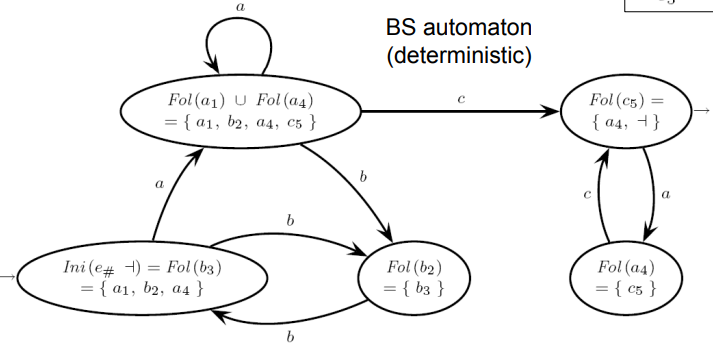
\includegraphics[width=0.8\linewidth]{images/BS.png}
    \end{figure}
\end{example}
Another use of algorithm BS is as an alternative to the power set construction, for converting a nondeterministic machine $N$ into a deterministic one $M$. The steps are: 
\begin{enumerate}
    \item Distinctly number the labels of non-$\varepsilon$ arcs of $N$, obtaining automaton $N^{'}$.
    \item Compute the local sets $Ini$, $Fin$, and $Fol$ for the language $L(N^{'})$. These can be easily derived from the transition graph, possibly exploiting the 
        identity $\varepsilon a=a\varepsilon=a$.
    \item Applying the BS construction to the sets $Ini$, $Fin$, and $Fol$, produce the deterministic automaton $M$.
\end{enumerate}